% $Header: /cvsroot/latex-beamer/latex-beamer/solutions/generic-talks/generic-ornate-15min-45min.de.tex,v 1.4 2004/10/07 20:53:08 tantau Exp $

\documentclass{beamer}

% Diese Datei enth�lt eine L�sungsvorlage f�r:


% - Vortr�ge �ber ein beliebiges Thema.
% - Vortragsl�nge zwischen 15 und 45 Minuten. 
% - Aussehen des Vortrags ist verschn�rkelt/dekorativ.



% Copyright 2004 by Till Tantau <tantau@users.sourceforge.net>.
%
% In principle, this file can be redistributed and/or modified under
% the terms of the GNU Public License, version 2.
%
% However, this file is supposed to be a template to be modified
% for your own needs. For this reason, if you use this file as a
% template and not specifically distribute it as part of a another
% package/program, I grant the extra permission to freely copy and
% modify this file as you see fit and even to delete this copyright
% notice. 



\mode<presentation>
{
  \usetheme{Singapore}
  % oder ...
  
  \setbeamercovered{transparent}
  % oder auch nicht
}


\usepackage[ngerman]{babel}
% oder was auch immer

\usepackage[latin1]{inputenc}
% oder was auch immer

\usepackage{times}
\usepackage[T1]{fontenc}
% Oder was auch immer. Zu beachten ist, das Font und Encoding passen
% m�ssen. Falls T1 nicht funktioniert, kann man versuchen, die Zeile
% mit fontenc zu l�schen.

\usepackage[]{textpos}


\title[] % (optional: Kurzversion, nur bei langen Titeln n�tig)
{Entwicklung eines Bootloader f�r �ber CAN verbundene Mikrocontroller}

%\subtitle
%{Untertitel} % (optional)

\author[] % (optional, nur bei vielen Autoren)
{J�rg Diederich}
% - Der \inst{?} Befehl sollte nur verwendet werden, wenn die Autoren
%   unterschiedlichen Instituten angeh�ren.

\institute[Universit�ten Hier und Dort] % (optional, aber oft n�tig)
{Institut f�r Verteilte Systeme\\
 AG Eingebettete Systeme und Betriebssysteme
}
% - Der \inst{?} Befehl sollte nur verwendet werden, wenn die Autoren
%   unterschiedlichen Instituten angeh�ren.
% - Keep it simple, niemand interessiert sich f�r die genau Adresse.

\date[Kurzversion des Anlass] % (optional)
{Sommersemester 2007}


\subject{Informatik}
% Dies wird lediglich in den PDF Informationskatalog einf�gt. Kann gut
% weggelassen werden.


% Falls eine Logodatei namens "university-logo-filename.xxx" vorhanden
% ist, wobei xxx ein von latex bzw. pdflatex lesbares Graphikformat
% ist, so kann man wie folgt ein Logo einf�gen:

% \pgfdeclareimage[height=0.5cm]{university-logo}{university-logo-filename}
\logo{
}

\titlegraphic{
  \begin{figure}[htbp]
    \begin{center}
      \scalebox{0.1}{
\includegraphics{../pics/ovg}}
    \end{center}
  \end{figure}
}

% Folgendes sollte gel�scht werden, wenn man nicht am Anfang jedes
% Unterabschnitts die Gliederung nochmal sehen m�chte.
\AtBeginSubsection[]
{
%  \begin{frame}<beamer>
%    \frametitle{Gliederung}
%    \tableofcontents[currentsection,currentsubsection]
%  \end{frame}
}


% Falls Aufz�hlungen immer schrittweise gezeigt werden sollen, kann
% folgendes Kommando benutzt werden:

%\beamerdefaultoverlayspecification{<+->}

%\setbeamertemplate{navigation symbols}{
%  \insertslidenavigationsymbol
%  \insertframenavigationsymbol 
%}





\begin{document}
%
\begin{frame}[plain]
  \begin{center}
  \color{structure}
  {\LARGE \inserttitle}
  \inserttitlegraphic
  \normalcolor
  \insertauthor\\[5mm]
  \normalsize
  Doktoranden- und Diplomandenseminar\\[1mm]
  \insertinstitute\\[2mm]
  \small \insertdate
\end{center}
\end{frame}

\begin{frame}
  \frametitle{Gliederung}
  \tableofcontents[pausesections]
  % Die Option [pausesections] k�nnte n�tzlich sein.
\end{frame}

\section{Einleitung}

\subsection[]{Ausgangssituation}

\begin{frame}
  \frametitle{In-System-Programming}
  
  \begin{columns}[t]
    \begin{column}{3cm}
      \vspace{0mm}
      \setbeamercolor{bl20w}{fg=black,bg=blue!20!white}
      \begin{beamercolorbox}[wd=3cm,rounded=true,shadow=true,dp=2ex]{bl20w}
        {\tiny Client}
        \\
        \centering Programmier-\\software
      \end{beamercolorbox}
    \end{column}
    \begin{column}{3cm}
      \vspace{3mm}
      \setbeamercolor{bl20w}{fg=black,bg=blue!20!white}
      \begin{beamercolorbox}[wd=3cm,rounded=true,shadow=true,center]{bl20w}
        Programmier-\\adapter
      \end{beamercolorbox}
    \end{column}
    \begin{column}{3cm}
      \vspace{0mm}
      \setbeamercolor{bl20w}{fg=black,bg=blue!20!white}
      \begin{beamercolorbox}[wd=3cm,rounded=true,shadow=true,dp=2ex]{bl20w}
        {\tiny Server}
        \\
        \centering Mikro-\\controller
      \end{beamercolorbox}
    \end{column}
  \end{columns}
  \begin{textblock}{3}(3.7,-2.2)
    \begin{figure}
      \scalebox{1.0}{
\includegraphics{../pics/arrow_right}}
    \end{figure}
  \end{textblock}
  \begin{textblock}{3}(8.7,-2.2)
    \begin{figure}
      \scalebox{1.0}{
\includegraphics{../pics/arrow_right}}
    \end{figure}
  \end{textblock}
  \vspace{5mm}
  \begin{itemize}
    \item Verwenden exisitierender und standardisierter I/O-Schnittstellen
      auf beiden Seiten
      \item Operationen umfassen L�schen, Schreiben und Lesen von bzw. in 
        unterschiedliche Speicherbereiche
  \end{itemize}
\end{frame}

\subsection[]{Problem und L�sungsm�glichkeit}

\begin{frame}
  \frametitle{Motivation}

  \setbeamersize{description width=0cm}
  \begin{description}
    \item Problem: \\
      \begin{itemize}
      \item minimale Anzahl von Kommunikationspartnern bei bisher 
        verwendeten Kommunikationswegen\\[1ex]
      \item Aufwand f�r ISP steigt mit zunehmender Anzahl zu bearbeitender 
        Mikrocontroller
      \end{itemize}
      \vspace{4mm}
    \item L�sungsm�glichkeit: \\
      \setbeamercolor{itemize item}{fg=green!80!black}
      \begin{itemize}
      \item Ausnutzen der existierenden Verbindung der Mikrocontroller �ber 
        Bussysteme\\
        \begin{description}
          \item \alert{CAN}, TWI
        \end{description}
      \end{itemize}
    \end{description}
\end{frame}


\section{Anforderungen}
\subsection[]{AVR}
\subsection[]{CAN-Verbindung}

\begin{frame}
  \frametitle{Anforderungen}

  \begin{description}
    \item AVR AT90CAN Mikrocontroller
      \begin{itemize}
      \item Bootloader-Support mit 8kByte Programmspeicher \\[1ex]
      \item integrierter CAN-Controller nach CAN 2.0B
      \end{itemize}
      \vspace{4mm}
      \begin{textblock}{3}(0,-3.5)
        \begin{figure}
          \scalebox{0.1}{
\includegraphics{../pics/logo_atmel_crop}}
        \end{figure}
      \end{textblock}
    \item CAN-Adapter
      \begin{itemize}
      \item Anbindung eines PC an einen CAN-Bus �ber Dongle oder 
        Steckkarte \\[1ex]
      \item Linux-Unterst�tzung mit Treiber und Library
      \end{itemize}
      \begin{textblock}{3}(0,-2.6)
        \begin{figure}
          \scalebox{0.1}{
\includegraphics{../pics/logo_peaksystem_crop}}
        \end{figure}
      \end{textblock}
  \end{description}
\end{frame}

\section{Vorgehen}
\subsection[]{Verwandte Arbeiten}

\begin{frame}
  \frametitle{Verwandte Arbeiten}

  \begin{columns}[t]
    \begin{column}{4,5cm}
      \vspace{0mm}
      \setbeamercolor{bl20w}{fg=black,bg=blue!20!white}
      \vspace{2mm}
      \begin{beamercolorbox}[wd=0cm,rounded=true,shadow=true,center]{bl20w}
        {\tiny Client}
      \end{beamercolorbox}
      avrdude
      \begin{itemize}
      \item (Standard-)Client mit verschiedenen Programmieradaptern
      \item Verwendung der seriellen (RS232) und parallelen Schnitt\-stellen 
        des PC
      \end{itemize}
    \end{column}
    \begin{column}{0,25cm}
    \end{column}
    \begin{column}{4,5cm}
      \setbeamercolor{bl20w}{fg=black,bg=blue!20!white}
      \vspace{2mm}
      \begin{beamercolorbox}[wd=0cm,rounded=true,shadow=true,center]{bl20w}
        {\tiny Server}
      \end{beamercolorbox}
      Atmel AN914
      \begin{itemize}
      \item Protokoll f�r CAN-Bus
      \item Geeignet f�r genau 1 Server
      \item Implementation f�r Windows
      \end{itemize}
    \end{column}
  \end{columns}

  \begin{textblock}{3}(5.7,-8.0)
    \begin{figure}
      \scalebox{1.0}{
\includegraphics{../pics/arrow_right_mov}}
    \end{figure}
  \end{textblock}

\end{frame}

\subsection[]{Bootloader}

\begin{frame}
  \frametitle{Entwicklung des Bootloaders}

  \setbeamersize{description width=0.3cm}
  \begin{itemize}
  \item Variation des in AN914 vorgeschlagenen Protokolls
    \begin{description}
    \item Identifier einer CAN-Nachricht kennzeichnet sendenden Knoten\\[1.4cm]
    \end{description}
  \item lediglich lose Kopplung aller beteiligten Komponenten des Bootloaders
    angestrebt
  \end{itemize}

  \begin{textblock}{3}(1.4,-3.6)
    \begin{figure}
      \scalebox{0.65}{\rotatebox{0}{
\includegraphics{../pics/protocol}}}
    \end{figure}
  \end{textblock}
  \vspace{2.5cm}

%  \framezoom<1><2>[border](5.2cm,4cm)(3.5cm,2.5cm)
  \framezoom<1><2>(5.2cm,4.2cm)(3.5cm,2.5cm)
  \begin{textblock}{3}(7.5,-4.2)
    \begin{figure}
    \scalebox{0.225}{\rotatebox{270}{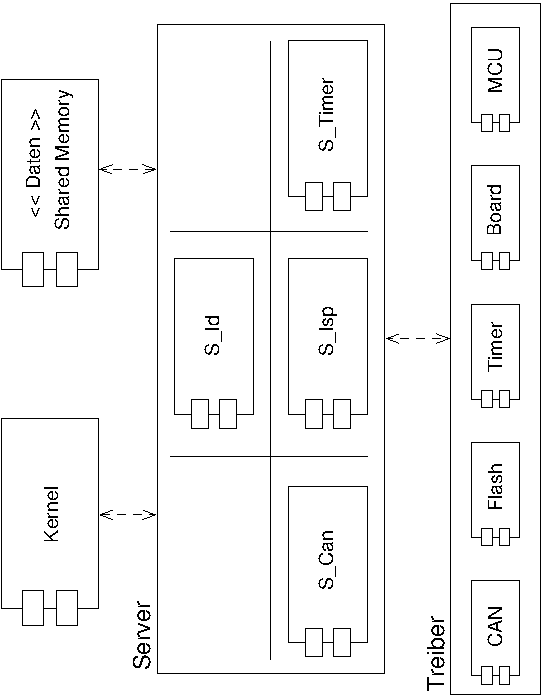
\includegraphics{../pics/komp_model_shumway}}}
    \end{figure}
  \end{textblock}
\end{frame}


\subsection[]{avrdude}

\begin{frame}
  \frametitle{Erweiterung von avrdude}

  \begin{columns}[t]
    \begin{column}{6.5cm}
      \setbeamersize{description width=0.3cm}
      \setbeamercolor{itemize item}{fg=green!80!black}
      \vspace{0.5cm}
      \begin{itemize}
      \item neuer Programmieradapter: shumway\\[0.1cm]
        \begin{description}
        \item Implementierung von call-backs\\[0.5cm]
        \end{description}
      \item neue Schnittstelle: CAN\\[0.1cm]
        \begin{description}
        \item Verwendung der libpcan
        \end{description}
      \end{itemize}
    \end{column}
    \begin{column}{5cm}
      \begin{figure}
        \scalebox{0.45}{\rotatebox{0}{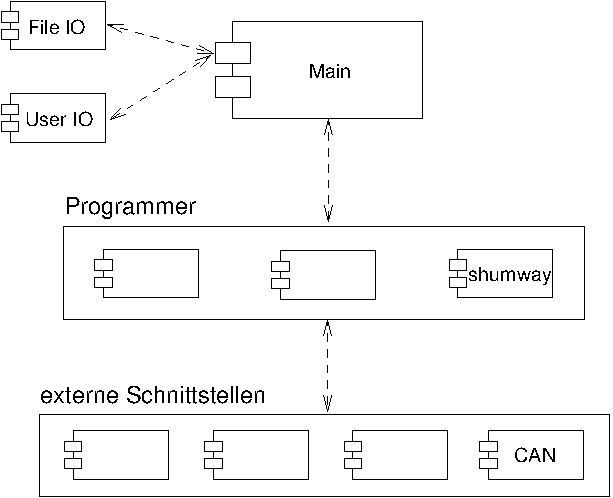
\includegraphics{../pics/komp_model_avrdude}}}
      \end{figure}
    \end{column}
  \end{columns}
  \vspace{1cm}
\end{frame}

\section*{Zusammenfassung}

\begin{frame}
  \frametitle<presentation>{Zusammenfassung}
  
  \setbeamersize{description width=0.3cm}
  \setbeamercolor{itemize item}{fg=red!50!yellow}
  \begin{itemize}
  \item Verwendung eines Protokolls f�r mehrere reaktive Knoten\\[0.2cm]
  \item Entwicklung und Implementierung eines Bootloaders\\[0.1cm]
    \setbeamercolor{itemize item}{fg=red!50!yellow}
    \begin{itemize}
        \item jede Instanz besitzt eindeutigen Identifier
        \item Abbruchbedingung nach Reset
        \item Ansprung aus Applikation vorbereitet
        \end{itemize}
  \item Fortgesetzte Anwendung von avrdude als Programmiersoftware\\[0.1cm]
    \begin{itemize}
      \item Geschwindigkeit Schreiben/Verify: ca. 1,5kB/s
    \end{itemize}

  \end{itemize}
\end{frame}

\begin{frame}
  \frametitle{Schwierigkeiten}

  \begin{enumerate}
    \item \alert{Codesize}\\[0.7cm]
    \item Asynchronit�t\\[0.7cm]
    \item Uabh�ngige Weiterentwicklung von avrdude\\[0.7cm]
  \end{enumerate}
\end{frame}

\begin{frame}
  \begin{center}
    Vielen Dank f�r die Aufmerksamkeit.
  \end{center}
\end{frame}


\end{document}


